% Threat-Shape — project report, Visual Analytics, Sapienza University of Rome.
%
% Compile with pdflatex (Overleaf: set the main document to this file). The figures are
% the screenshots in docs/img, reached through \graphicspath below, so the folder layout
% of the repository is enough - nothing needs copying.
%
% Samuele Proietti and Marco Alberti, group project.

\documentclass[conference]{IEEEtran}

\usepackage{graphicx}
\usepackage{booktabs}
\usepackage{amsmath}
\usepackage[hidelinks]{hyperref}
\usepackage{url}

\graphicspath{{../img/}{img/}}

\begin{document}

\title{Threat-Shape: Visual Analytics for the Shape\\of a National Cyber-Threat Profile}

\author{
\IEEEauthorblockN{Samuele Proietti}
\IEEEauthorblockA{Sapienza University of Rome\\
proietti.1946329@studenti.uniroma1.it}
\and
\IEEEauthorblockN{Marco Alberti}
\IEEEauthorblockA{Sapienza University of Rome\\
alberti.1794463@studenti.uniroma1.it}
}

\maketitle

\begin{abstract}
Public cyber-incident repositories are usually explored by counting: how many incidents
a country suffered, in which year, of which type. Counting answers how much, never what
kind. Threat-Shape is a visual analytics tool that moves a threat-intelligence analyst
from the volume of a national threat profile to its \emph{composition} --- which sectors,
techniques and actors define it, and how it departs from another country's or from the
global expectation. It couples four bidirectionally coordinated views over the 3{,}414
incidents of the European Repository of Cyber Incidents (EuRepoC) with three computations
that run only in response to a visual gesture: a standardized deviation per country, a
t-SNE re-projection refitted on the selected subset alone, and a contrastive
two-proportion test that ranks the indicators separating a selection from its comparison.
Used on the corpus, the tool splits the incidents targeting Russia into two operational
families that differ by a factor of two in intensity while sharing the same attackers,
shows that attribution rates track the adversary mix rather than the victim's forensic
capability, and exposes a coding-coverage break in the source data that would otherwise
be read as a change in the threat itself.
\end{abstract}

\begin{IEEEkeywords}
visual analytics, coordinated views, dimensionality reduction, t-SNE, cyber threat
intelligence, contrastive analysis
\end{IEEEkeywords}

\section{Introduction}

A threat-intelligence analyst at a national CSIRT preparing a situational assessment does
not primarily need to know \emph{how many} incidents a country suffered. That number is
already published. What the assessment turns on is the \emph{shape} of the threat: which
sectors are hit more than the global mix would predict, which operations and access
vectors recur, whether the adversary is a state, a criminal group or a volunteer, and how
all of this differs from a peer nation's profile.

Public repositories and their dashboards are organised around the first question. They
filter and they count, so an analyst who wants the second question answered is left to
export the data and write code --- which is exactly the loop visual analytics exists to
close.

Threat-Shape is our answer. Its contributions are:

\begin{itemize}
\item a four-view coordinated interface over the EuRepoC corpus in which the projection
of incident \emph{profiles} is the organising view rather than a decoration;
\item three analytics that are computed on the live selection and are reachable only
through a visual gesture --- no menu produces a result, and no result exists before an
interaction;
\item a contrast panel that reports both rates being compared, grouped into the six
questions an analyst asks of a profile, with an explicit reliability test rather than a
ranking by raw magnitude;
\item five findings obtained with the tool, including one about the source data itself,
and a verification suite that re-checks the interaction contract on demand.
\end{itemize}

\section{Related Work and Positioning}

\subsection{The reference solution: the EuRepoC dashboard}

Our data and our closest competitor come from the same project. EuRepoC codes publicly
reported, politically relevant cyber incidents against roughly sixty criteria assessed by
experts in IT forensics, political science and international law~\cite{eurepoc-data},
and publishes an official interactive dashboard over the same corpus~\cite{eurepoc-dash}.

That dashboard is built for volume and filtering: incident counts by country, by year, by
type and by sector, with a table view for individual incidents. Every question it answers
has the form \emph{how many, where, when}. The composition of a profile --- what makes
Italy's incidents different from Germany's once their different sizes are accounted for
--- is not among them, and neither is any form of dimensionality reduction. Threat-Shape
deliberately does not reproduce its counting views; the timeline is the only overlap, and
it is present as the temporal filter that restricts the three analytics rather than as an
answer in itself.

\subsection{Studies on the same corpus}

The corpus is also used in quantitative political science. Akoto et al.~\cite{akoto}
build a country--year panel over 195 countries (2000--2022) whose cyber-security outcomes
are taken from EuRepoC, in order to test whether data-localization policies improve those
outcomes. The contrast is instructive: there the same records are reduced to a handful of
country-level indicators for a regression, a treatment that answers one pre-registered
question well and is the opposite of what an analyst needs when the question is not yet
formed. Threat-Shape keeps the incident as the unit of analysis and lets the question be
posed by selection.

\subsection{Visual analytics for cyber security}

Surveys of the field show its centre of gravity is network traffic: Shiravi et
al.~\cite{shiravi} organise nearly all systems of the last two decades into five use-case
classes built on packets, flows and hosts. Threat-Shape sits elsewhere, on curated
incident records with political and legal coding, where an ``event'' is a documented
campaign rather than a packet capture.

Closer to us in data type, Böhm et al.~\cite{bohm} present a graph-based visual analytics
concept for semi-structured cyber threat intelligence, where analysts explore and enrich
threat information as a node-link structure. The shared premise is that threat
intelligence is worth exploring visually rather than tabulating; the difference is the
question. A graph answers \emph{what is connected to what}; our projection answers
\emph{what resembles what}, which is the question a profile poses.

\subsection{Interactive dimensionality reduction}

Sacha et al.~\cite{sacha} survey how analysts interact with dimensionality reduction and
find seven recurring interaction scenarios, of which the one we implement --- recomputing
a projection on a subset chosen in the view --- is among the most demanding, because the
result must remain interpretable when the subset gets small. We use t-SNE~\cite{tsne},
report its trustworthiness~\cite{venna} with every local re-projection, and follow the
warnings collected by Wattenberg et al.~\cite{misread} about how its pictures are
misread; they drove concrete decisions in Section~\ref{sec:design}.

\subsection{Coordination and comparison}

The coordination model follows the classic multiple-view literature~\cite{roberts}: one
shared selection, every view both a source and a target, no view talking to another
directly. For the contrast panel we follow Gleicher et al.'s taxonomy of visual
comparison~\cite{gleicher}: our design is an explicit encoding of the difference (the
segment length) superimposed on a juxtaposition of the two rates (the two dots), which is
what lets the panel state both the effect size and the levels it is computed from.

\subsection{What is different here}

Counting tools answer volume; graph tools answer connection; projection tools rarely make
the projection the entry point to per-feature statistics. Threat-Shape puts the three
together: a selection made on a map, a projection or a timeline parameterises three
statistics that are reported back into the same views, and the projection itself is
refitted on that selection so that structure the global embedding had to compress can
re-emerge.

\section{Data}

\subsection{Source and unit of analysis}

EuRepoC ships four relational tables joined on \texttt{incident\_id}. The release we use
contains 3{,}414 incidents (2000--2024) in the global table, with 4{,}296
initiator--receiver pairs, 5{,}217 attribution claims and 12{,}180 targeted
entities~\cite{eurepoc-data}. The incident is our unit of analysis.

\subsection{Column selection and the AS index}

Of the 85 columns of the global table, most are identifiers, source URLs, free text or
update metadata. A verification pass over the real files retained \textbf{18 analytical
columns}: 14 categorical blocks (incident type, initial access, impact technique,
functional and intelligence impact, cyber and offline conflict issue, international-law
indicator, initiator category, state responsibility, receiver category, data theft,
disruption, hijacking) and 4 ordinal severity variables. The AS index is therefore

\[
3{,}414 \text{ tuples} \times 18 \text{ dimensions} = 61{,}452 .
\]

This is above the 10{,}000--50{,}000 band, deliberately and with the course's ``and more
for the braves'' allowance in mind. The count is of \emph{conceptual} variables: the same
18 columns expand into 123 binary indicators once their multi-valued cells are exploded,
which with the 4 ordinals gives the 127-column matrix the projection is computed on.
Quoting the exploded width as the AS index would inflate it to over 430{,}000 and would
describe the encoding rather than the data.

\subsection{Encoding and missing values}

Multi-valued cells (EuRepoC separates repeated values with semicolons, including inside
parenthesised explanations, which a naive split corrupts) are exploded into one binary
indicator per category. ``Not available'' is kept as its own indicator rather than
dropped: whether a field was coded is itself a signal, and Section~\ref{sec:insights}
shows a finding that exists only because those indicators were preserved. Columns are
standardized before PCA, because the binary matrix has strongly non-uniform column
variance.

\subsection{Projection pipeline}

The 127-column matrix is reduced by PCA to 20 components (50.7\% of the variance
retained), then by t-SNE to two dimensions. PCA is static, offline denoising and is never
recomputed; t-SNE is the technique integrated in the interactive analysis flow. The global
embedding uses perplexity 30, chosen by the highest trustworthiness among the candidates
15, 30 and 50 (0.9877, \textbf{0.9897}, 0.9885 at $k=20$); KL divergence was deliberately
not the selection criterion, since it falls with perplexity by construction. The seed is
fixed, so the view is identical across restarts.

\section{Design}\label{sec:design}

\begin{figure*}[t]
\centering
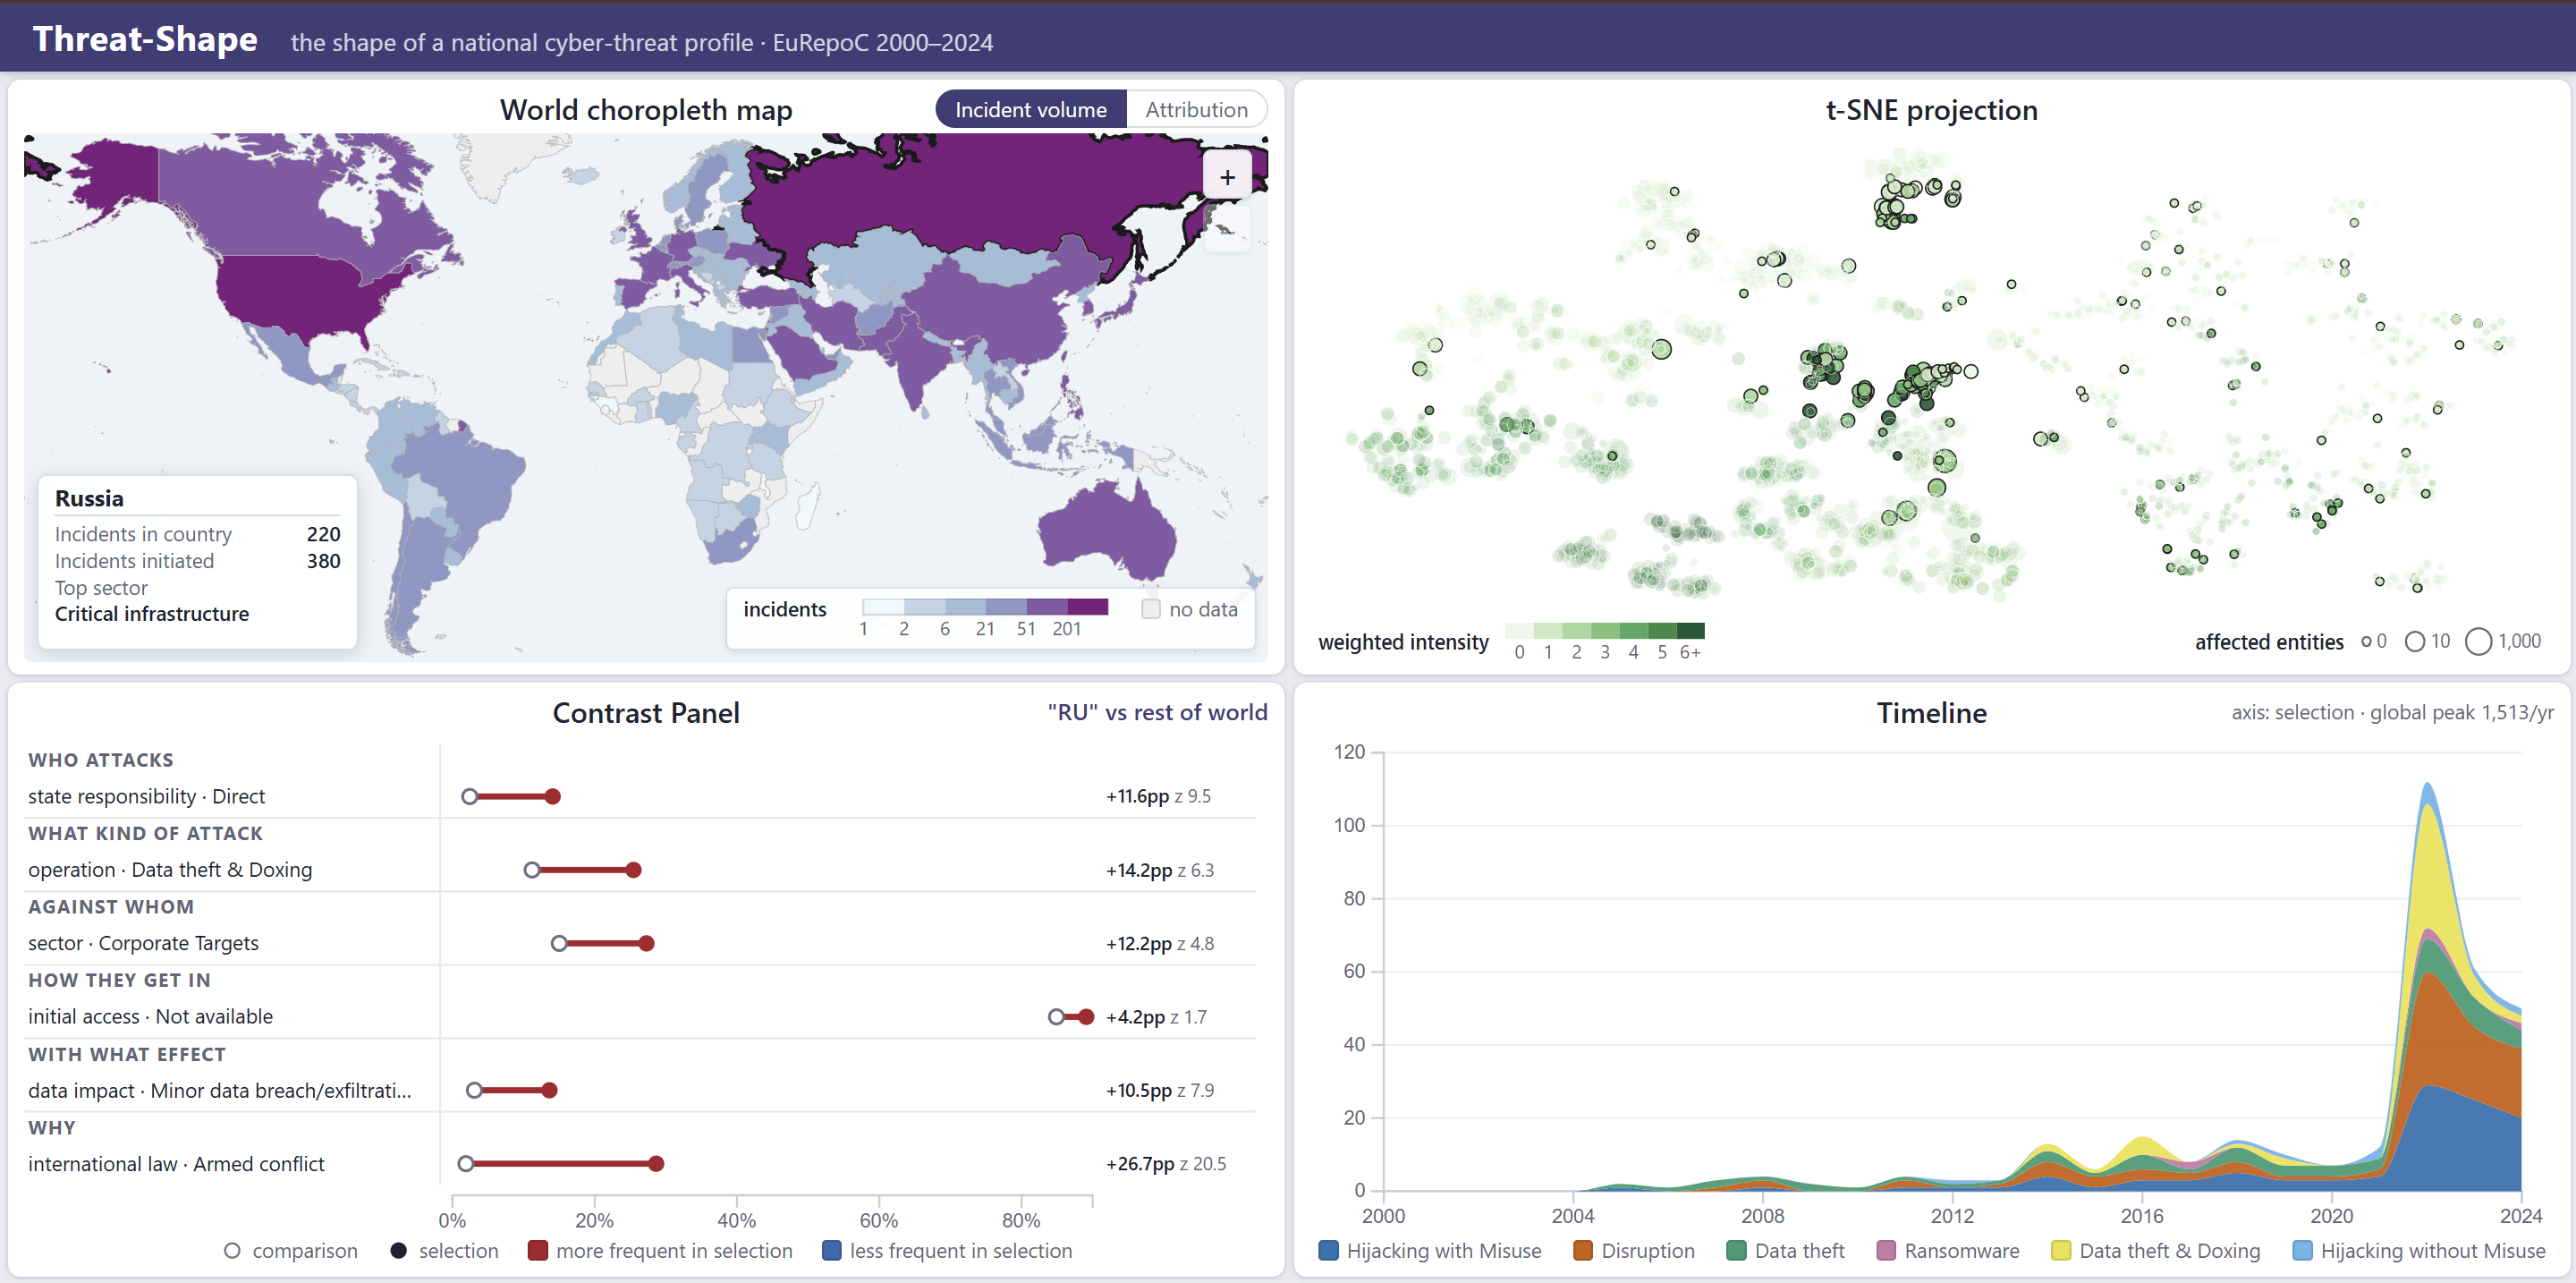
\includegraphics[width=\textwidth]{insight-1a-russia-two-clusters.png}
\caption{The four coordinated views after one click on Russia. The map reports 220
incidents suffered and 380 initiated; the projection highlights the Russian incidents
and shows them concentrating in two dense regions; the contrast panel states the
comparison in force; the timeline rescales its count axis to the selection and keeps the
global peak on screen as a number.}
\label{fig:overview}
\end{figure*}

Fig.~\ref{fig:overview} shows the interface. Four views share one selection state, and
each is both a source and a target of interaction.

\textbf{View A --- world choropleth.} The entry view. Clicking a country, or
ctrl-clicking several, drives the shared selection; a details panel reports the incidents
suffered, the incidents initiated and the most targeted sector. A two-state switch
replaces the layer with the share of incidents having no named initiator state. The
projection is Miller cylindrical, chosen after measuring two alternatives on the real
layout: an equal-area one made Europe --- where the corpus is densest and the countries
smallest --- hard to read and to click, while Mercator stretched the north until a
dashboard-shaped card had to crop Scandinavia. Miller is neither conformal nor
equal-area, which we state rather than hide.

\textbf{View B --- t-SNE projection.} One mark per incident, colour on a sequential
single-hue ramp for weighted intensity, and size on $\log(1+x)$ of the affected entities
with the value on the \emph{area} rather than the radius, since area ratios are estimated
badly. Following~\cite{misread}, no axis is drawn or labelled and the caveat that
inter-cluster distances carry no meaning is attached to the view. A free lasso is the
gesture that triggers the local re-projection.

\textbf{View C --- stacked area timeline.} Incident types per year, on the
colour-vision-safe Okabe--Ito palette; the seven atomic types are under the twelve a
categorical palette can carry, so no regrouping was needed. Brushing restricts every
analytic to the window. The count axis follows the selection \emph{without} its time
filter, so dragging the brush does not rescale the chart under the analyst's hand: a
window is a window onto a series, and it has to stay comparable with the years outside it.

\textbf{View D --- contrast panel.} One row per indicator, grouped into the six questions
of a profile: who attacks, what kind of attack, against whom, how they get in, with what
effect, why. Each row is a dumbbell: a hollow dot for the comparison group's rate, a
filled dot for the selection's, and a segment whose length is the difference and whose
colour is its sign. Reporting both rates is a deliberate correction of an earlier bar
design: a difference of $+22.7$ percentage points says nothing about whether it runs from
8\% to 31\% or from 57\% to 80\%.

Two rules cut across the design. Divergent colour is used only where a sign is meaningful
(the residual map, the contrast segments) and sequential colour everywhere else; and every
view carries its own legend, placed inside the chart where the data leaves space, so that
no legend costs the chart height.

\section{Analytics}

None of the three computations may run before a selection exists. On load the contrast
panel is empty by construction, and the analytics endpoints refuse a request without a
selection, so no typed URL can produce a ``global'' result.

\subsection{Standardized deviation}

For the country--sector contingency of the current selection, the observed proportion is
standardized against the expected one, $z=(x-\mu)/\sigma$. The map recolours on $z$ with a
divergent scale. Cells whose expected frequency falls below 5 are \emph{flagged} with
hatching and a ``small sample'' badge rather than suppressed: hiding them would leave the
analyst unable to tell a reliable zero from an unreliable one. The residual is computed
over the selection minus its country filter, because asking which countries are unusual
inside a selection defined by picking countries is circular --- measured, picking Italy
alone made Italy 100\% of its own selection against an expected 3\%.

\subsection{Local re-projection}

A lasso refits t-SNE on the enclosed incidents alone, with the same seed and a perplexity
adapted to the subset, $(n-1)/3$ capped at 30. Below 30 incidents the request is refused
with a message instead of an embedding. The threshold is measured, not assumed: repeated
random subsets show the spread of trustworthiness across subsets of the same size
halving between $n=15$ and $n=30$, so 30 is where the layout becomes \emph{reproducible},
not where it becomes good. Every accepted re-projection reports its $n$, its perplexity
and its trustworthiness in a banner, because a local layout and the global one look alike
while their axes mean different things.

\begin{figure}[t]
\centering
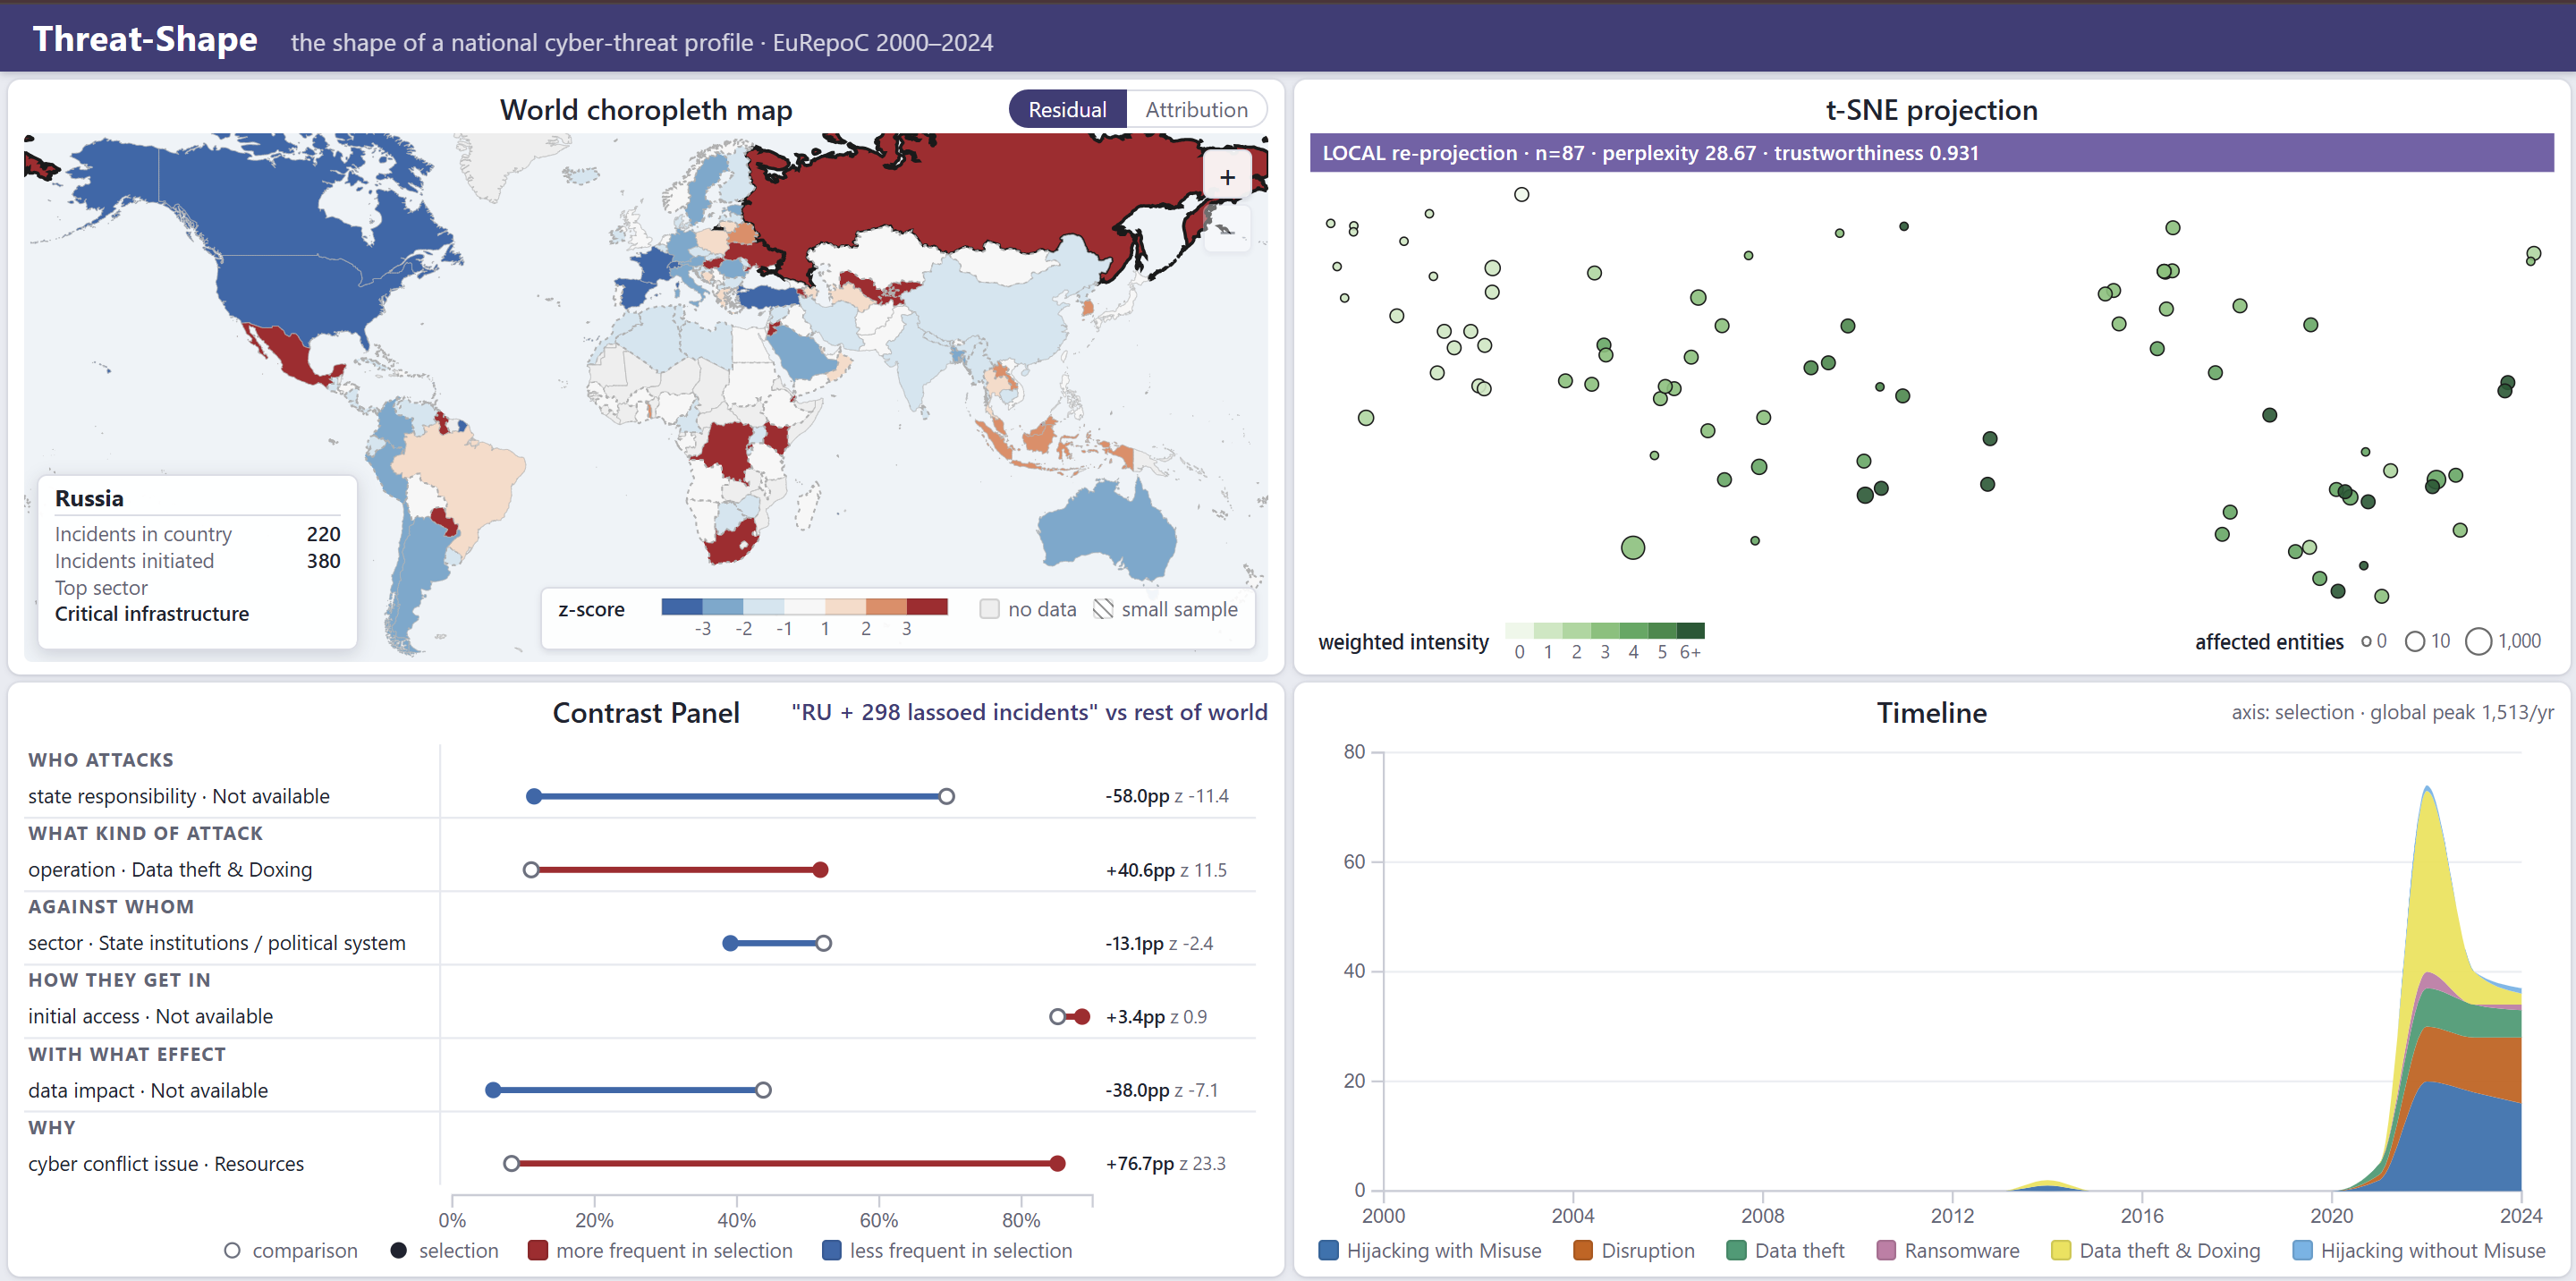
\includegraphics[width=\columnwidth]{insight-1b-russia-reprojected.png}
\caption{The dimensionality reduction inside the analysis flow. A lasso over the Russian
cluster refits t-SNE on the enclosed incidents alone; the banner states that the layout is
local and reports $n$, the adapted perplexity and the trustworthiness of the new
embedding. The other views follow the same selection: the map switches to the standardized
deviation and the contrast panel recomputes.}
\label{fig:reproject}
\end{figure}

\subsection{Contrastive z-scores}

For each of the 123 indicators, the proportion carrying it in the selection is compared
with the proportion in the comparison group by a pooled two-proportion $z$-test. The
comparison group is the complement of the selection, except when exactly two countries are
selected, where it becomes the second country --- with three or more there is no
well-defined ``B'' to nominate, as measured: contrasting $\{$IT, DE, FR$\}$ with each
member in turn as the pivot shares none of the top five features between two of the three
pivots.

Bar length and ranking encode different quantities on purpose. The segment length is the
difference in percentage points, an effect size; the ranking is by $|z|$, which weighs how
many incidents that difference rests on. A feature that differs hugely across six
incidents draws a long segment and sinks in the list. Features failing the validity
condition of the normal approximation are shown faded and dashed rather than removed, and
a group below 20 incidents is refused outright.

\section{Insights}\label{sec:insights}

Five findings are documented, each reachable by a gesture, produced by one of the three
analytics and reported with its $z$; $|z|\geq 2$ is our threshold for ``more than noise''
and figures below it are quoted as such. A script recomputes every number by calling the
same endpoints the interface calls.

\subsection{Russia splits into two operational families}

Selecting Russia (220 incidents as a receiver) concentrates the highlighted marks in two
dense regions of the projection. Lassoing each in turn gives a mean weighted intensity of
1.59 against 3.26. Contrasted against the other Russian incidents, the first is defined by
an impact lasting a single day ($+73.5$ pp, $z=10.8$) with no data breach, the second by
data exfiltration ($+65.9$ pp, $z=10.0$) and by an offline conflict over territory and
resources. Both re-project reliably (trustworthiness 0.938 and 0.977).

The two families are \emph{not} separated by attacker: Ukraine's military intelligence and
volunteer groups appear in both, and the share with no named initiator state is 38\%
against 40\%. The projection cut by what the operation does and how deep it gets --- the
cut a defender needs, and one no actor-based grouping would produce.

\subsection{A coding break masquerading as a trend}

\begin{table}[t]
\caption{Coverage of three EuRepoC blocks by year, as the tool reports it. The break
between 2019 and 2023 dominates any contrast that spans it.}
\label{tab:coverage}
\centering
\begin{tabular}{@{}lrrrr@{}}
\toprule
Year & $n$ & law n/a & downtime n/a & types per incident \\
\midrule
2013 & 147 & 100.0\% & 100.0\% & 1.21 \\
2016 & 166 & 98.8\%  & 98.8\%  & 1.35 \\
2019 & 91  & 86.8\%  & 85.7\%  & 1.71 \\
2020 & 71  & 54.9\%  & 56.3\%  & 1.75 \\
2022 & 354 & 16.7\%  & 12.1\%  & 1.62 \\
2024 & 700 & 2.1\%   & 0.3\%   & 2.04 \\
\bottomrule
\end{tabular}
\end{table}

Brushing 2000--2013 returns five ``strongest'' features that are all artefacts of coding
(Table~\ref{tab:coverage}): fields that were simply not filled in the early years, at
$|z|$ between 26 and 34. Two things move at once across the break --- empty fields start
being coded, and the number of type labels attached to one incident grows from 1.21 to
2.04 --- so part of the timeline's dramatic rise is growth in coding granularity rather
than in the threat.

This is a finding about the data, produced by the tool's own contrast panel, and at the
same time a trap the same panel sets: a brush spanning the break answers a question about
editorial practice while looking like an answer about cyber conflict. The working rule we
adopted is to compare characteristics only inside the homogeneous era.

\subsection{Attribution follows the adversary, not the victim}

On the attribution layer the countries with at least 45 incidents fall into two regimes:
below 30\% unattributed (KR 17\%, SA 21\%, AE 24\%, IN, CN, VN, UA) and above 55\% (FR
72\%, ES, MX, CA, IT, US, DE, CH, AU, BE). The contrast panel explains the split: the mean
share of incidents with a state-affiliated initiator is 45.2\% in the first group against
15.6\% in the second. The intuitive hypothesis --- that western states with mature CERTs
attribute better --- is backwards; what differs is who attacks them.

\begin{figure}[t]
\centering
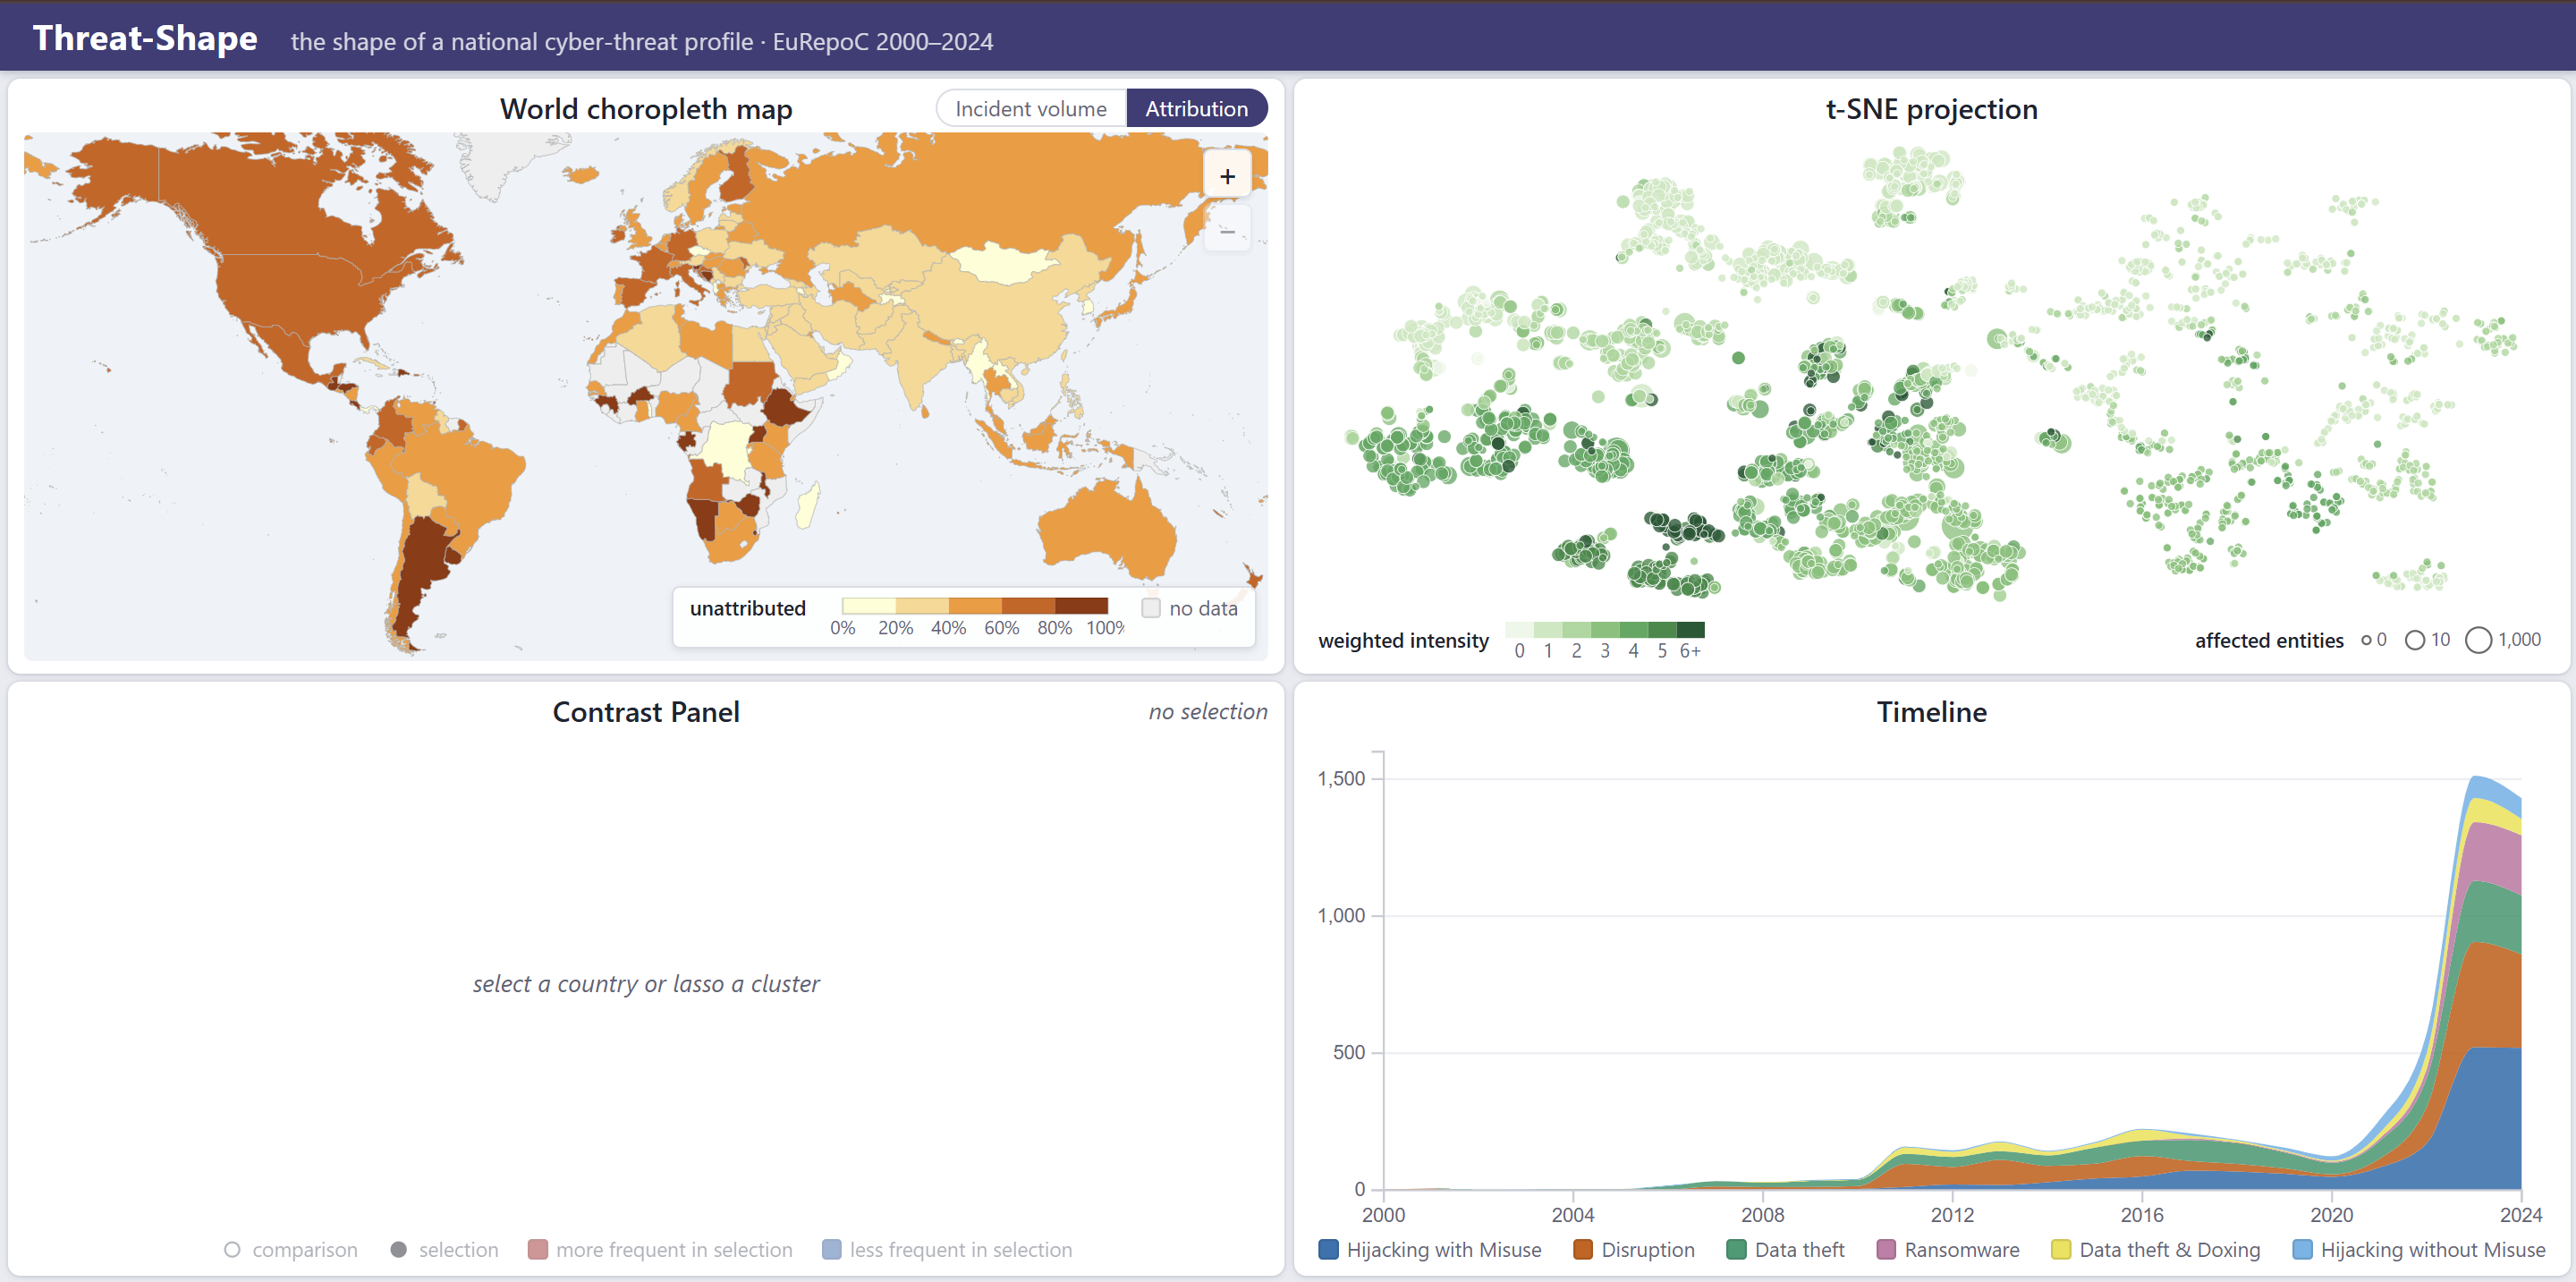
\includegraphics[width=\columnwidth]{insight-3-attribution-regimes.png}
\caption{The attribution layer, the second state of the map's display switch. The
sequential scale reports the share of a country's incidents with no named initiator
state, and separates the two regimes discussed here. No selection is active, so the three
analytics have produced nothing --- the contrast panel shows its prompt instead of a
result.}
\label{fig:attribution}
\end{figure}

\subsection{Ukraine and Russia are mirror images}

Selecting both countries switches the panel to a direct comparison
(Fig.~\ref{fig:uaru}). Ukraine is attacked by states (36.5\% against 10.4\%, $z=5.79$),
Russia by non-state groups (53.0\% against 13.1\%, $z=-7.46$) who publish what they steal
(doxing 27.2\% against 5.8\%). The same war produces two different threat profiles.

\begin{figure}[t]
\centering
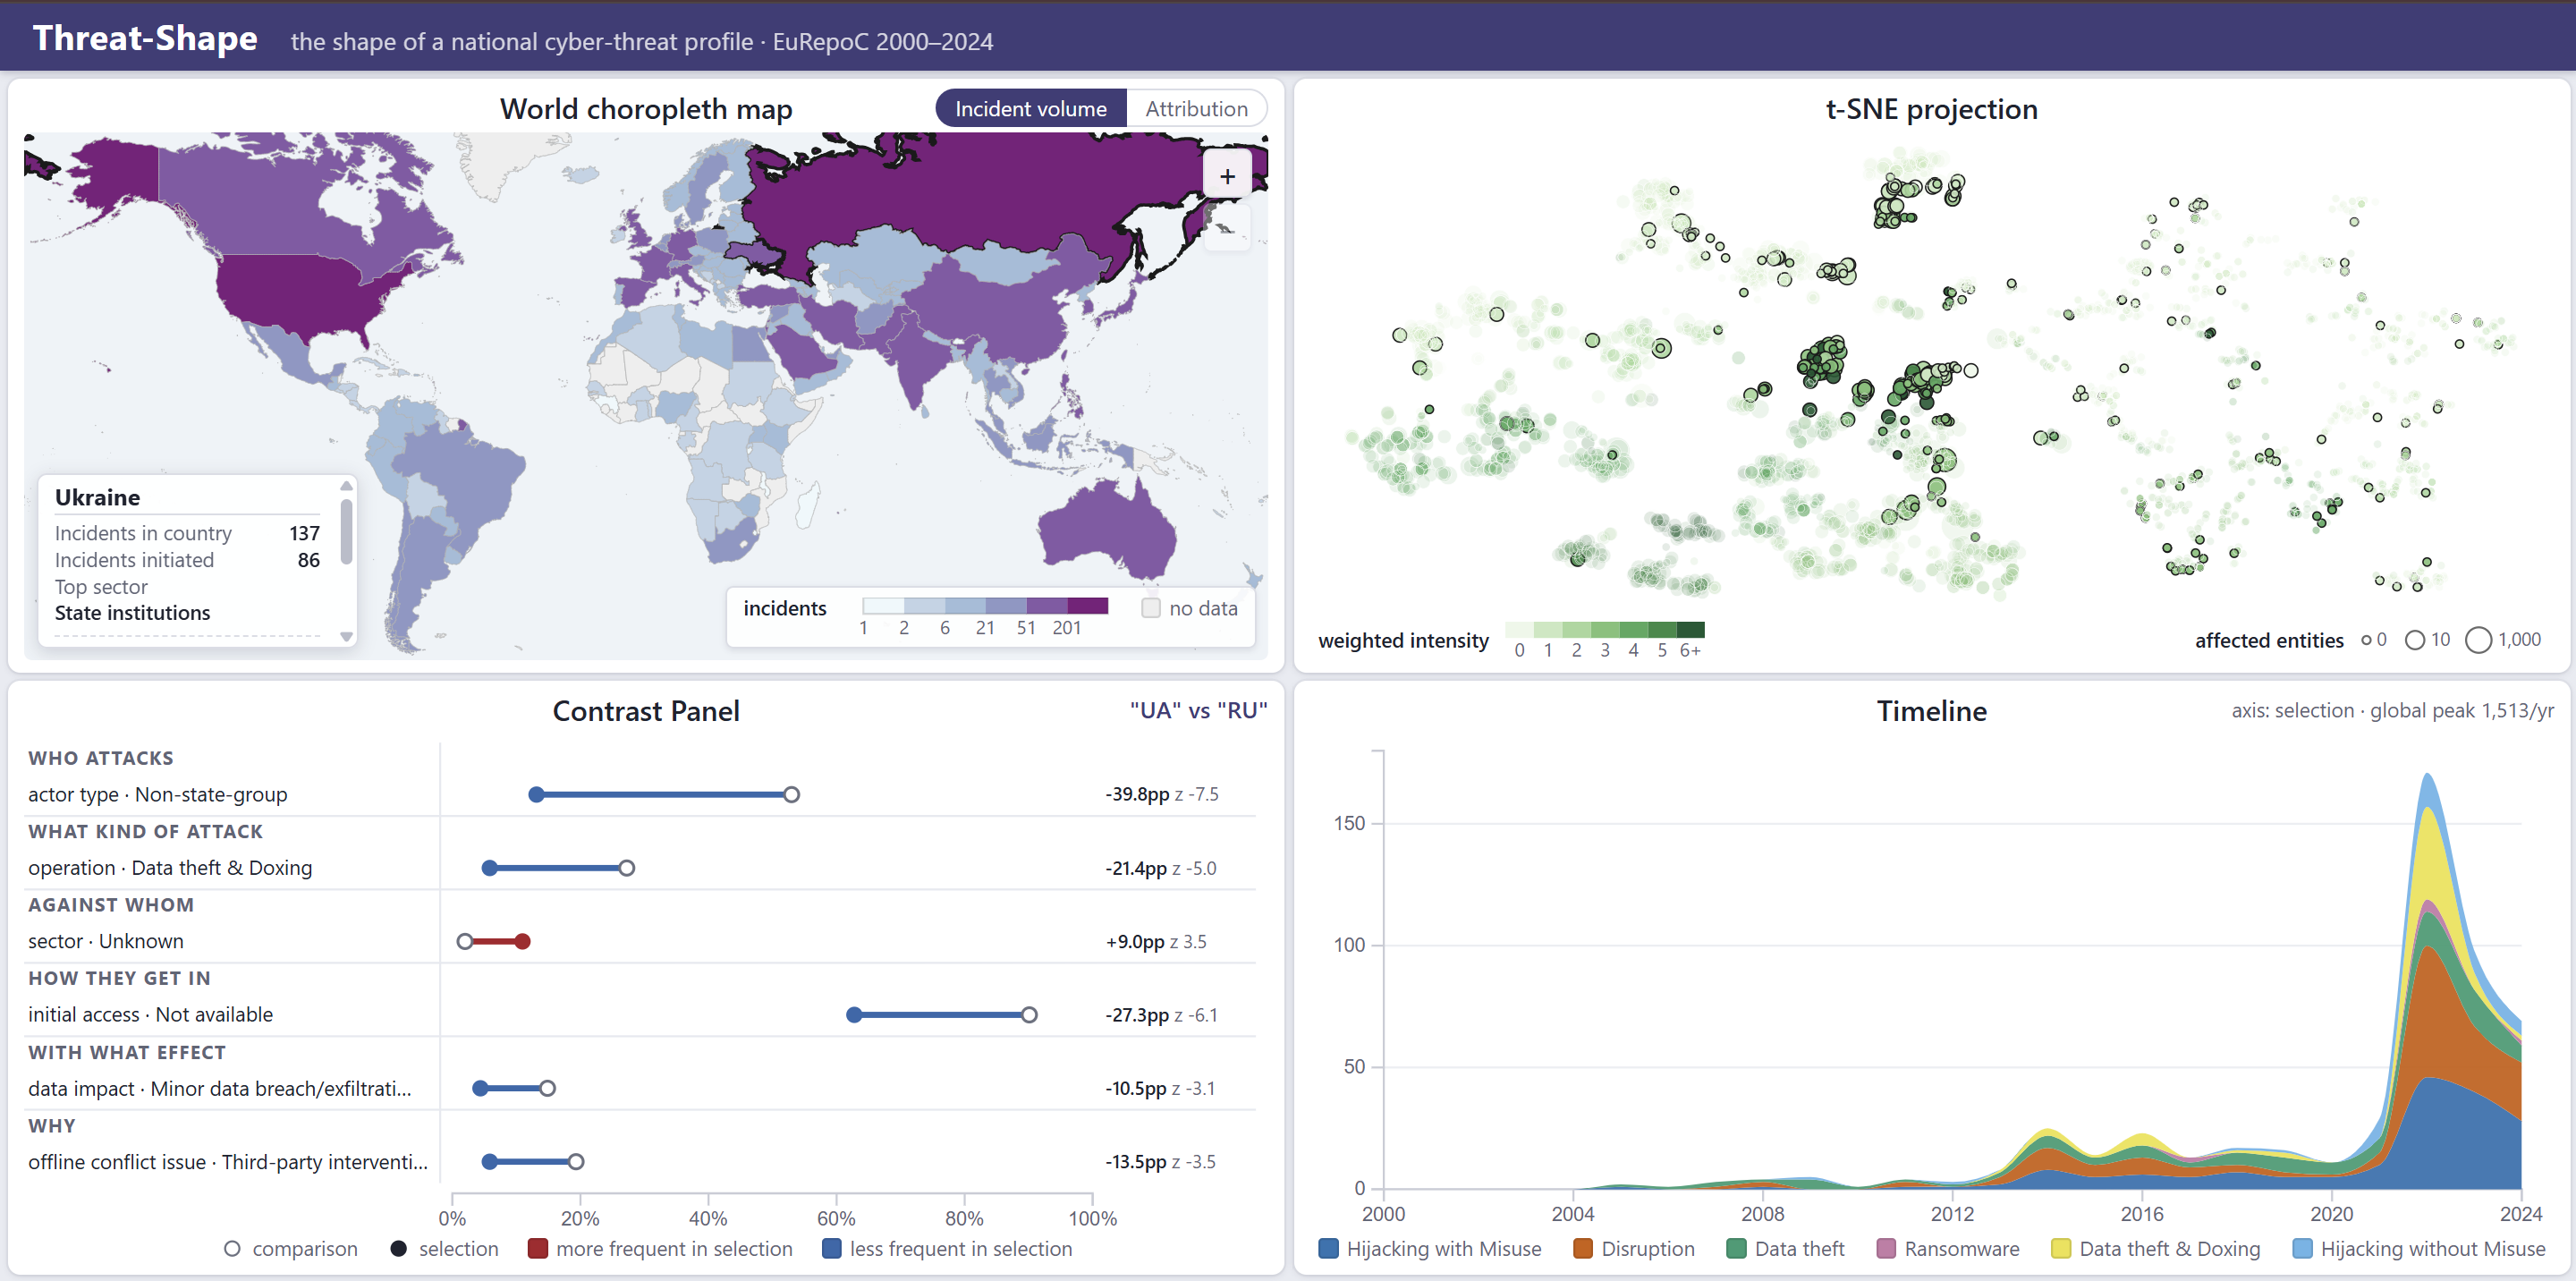
\includegraphics[width=\columnwidth]{insight-4-ukraine-russia.png}
\caption{Direct comparison mode: Ukraine against Russia. The panel states the comparison
in force, and each row reports both rates.}
\label{fig:uaru}
\end{figure}

\subsection{Italy against Germany}

Italian incidents are attributed to identifiable non-state groups two and a half times
more often than German ones (46.9\% against 18.6\%, $z=4.59$), with no state held
responsible, while half of the German incidents are attributed to nobody at all (49.4\%
against 25.9\%, $z=-3.47$). Against the rest of the world Italy shows critical
infrastructure at 61.7\% (against 40.0\%) and ransomware at 27.2\% (against 14.4\%). For a
CSIRT the difference is operational: a trackable criminal ecosystem on one side, a
documentation gap on the other.

\section{Verification}

Because two of the graded properties of this project are negative claims --- no analytic
is started by a menu, and no result exists before an interaction --- we made them
checkable rather than asserted. Four suites run on demand: a static audit of the sources
(no \texttt{select} or radio elements anywhere; each store mutator called from exactly one
view; the analytics endpoints answering 404 to GET and 422 to an empty selection), a
static audit of the visual encodings (palettes measured against three simulated
colour-vision deficiencies, divergent scales only on signed quantities, a legend in every
view), and two runtime suites driven from the browser console that replay interactions and
assert what is on screen. They currently report 26/26, 46/46, 25/25 and 34/34.

The suites have repeatedly earned their keep: they caught a plain click in the projection
that re-projected a country selection, and a redraw-on-resize implementation that reached
the views directly instead of going through the shared store --- reported as ``8 calls
found'' against the four the contract allows.

\section{Limitations}

The corpus records \emph{publicly reported} incidents, coded by humans; under-reporting is
invisible to the tool, and Section~\ref{sec:insights} shows how strongly coding practice
can drive a result. Each contrast tests 123 indicators without a multiple-comparison
correction, which is why our claims lean on $|z|>3$ and on features that agree with each
other. Initiators are not a map layer: the mirror-image finding had to be read through the
contrast panel rather than seen geographically. Finally, a bloc of three or more countries
is compared against the rest of the world as a group, with no per-member breakdown.

\section{Conclusion}

Threat-Shape shows that a curated incident corpus supports questions its own official
dashboard does not ask. By making the projection of incident profiles the organising view,
and by attaching three statistics to the gestures made on it, the tool answers what a
national threat profile is \emph{made of} rather than how large it is. The findings in
Section~\ref{sec:insights} --- two operational families behind one country's incident
count, an attribution pattern that inverts the intuitive explanation, and a coding break
that any purely count-based reading would have mistaken for a trend --- are the argument
that the distinction matters.

\begin{thebibliography}{99}

\bibitem{eurepoc-data}
K. Zettl-Schabath, J. Bund, M. Müller, C. Borrett, J. Hemmelskamp, A. Alibegovic,
E. Bajra, A. Jazxhi, E. Kellenter, A. Sachs, and C. Shelley,
``Global Dataset of Cyber Incidents (1.3.2),'' European Repository of Cyber Incidents,
2025. doi:10.5281/zenodo.14965395

\bibitem{eurepoc-dash}
European Repository of Cyber Incidents, ``Cyber Incident Dashboard.''
\url{https://eurepoc.eu/dashboard/} (accessed Sep. 2026).

\bibitem{akoto}
W. Akoto, S. Bradshaw, and T. Herr, ``Do data localization policies really improve
cybersecurity outcomes?,'' \emph{Journal of Cybersecurity}, vol. 12, no. 1,
art. tyag025, 2026.

\bibitem{shiravi}
H. Shiravi, A. Shiravi, and A. A. Ghorbani, ``A survey of visualization systems for
network security,'' \emph{IEEE Trans. Vis. Comput. Graph.}, vol. 18, no. 8,
pp. 1313--1329, 2012.

\bibitem{bohm}
F. Böhm, F. Menges, and G. Pernul, ``Graph-based visual analytics for cyber threat
intelligence,'' \emph{Cybersecurity}, vol. 1, no. 1, art. 16, 2018.

\bibitem{sacha}
D. Sacha, L. Zhang, M. Sedlmair, J. A. Lee, J. Peltonen, D. Weiskopf, S. C. North, and
D. A. Keim, ``Visual interaction with dimensionality reduction: A structured literature
analysis,'' \emph{IEEE Trans. Vis. Comput. Graph.}, vol. 23, no. 1, pp. 241--250, 2017.

\bibitem{tsne}
L. van der Maaten and G. Hinton, ``Visualizing data using t-SNE,'' \emph{J. Mach. Learn.
Res.}, vol. 9, pp. 2579--2605, 2008.

\bibitem{venna}
J. Venna and S. Kaski, ``Local multidimensional scaling,'' \emph{Neural Networks},
vol. 19, no. 6, pp. 889--899, 2006.

\bibitem{misread}
M. Wattenberg, F. Viégas, and I. Johnson, ``How to use t-SNE effectively,''
\emph{Distill}, 2016. doi:10.23915/distill.00002

\bibitem{roberts}
J. C. Roberts, ``State of the art: Coordinated and multiple views in exploratory
visualization,'' in \emph{Proc. 5th Int. Conf. Coordinated and Multiple Views in
Exploratory Visualization (CMV)}, 2007, pp. 61--71.

\bibitem{gleicher}
M. Gleicher, D. Albers, R. Walker, I. Jusufi, C. D. Hansen, and J. C. Roberts, ``Visual
comparison for information visualization,'' \emph{Information Visualization}, vol. 10,
no. 4, pp. 289--309, 2011.

\end{thebibliography}

\end{document}
